\documentclass[paper=a4, fontsize=11pt]{scrartcl} % A4 paper and 11pt font size

\usepackage[T1]{fontenc} % Use 8-bit encoding that has 256 glyphs
\usepackage{fourier} % Use the Adobe Utopia font for the document - comment this line to return to the LaTeX default
\usepackage[english]{babel} % English language/hyphenation
\usepackage{amsmath,amsfonts,amsthm} % Math packages

\usepackage[UTF8]{ctex}
%%%%%%%%%%%%%Python
\usepackage{listings}
\usepackage{color}

\definecolor{dkgreen}{rgb}{0,0.6,0}
\definecolor{gray}{rgb}{0.5,0.5,0.5}
\definecolor{mauve}{rgb}{0.58,0,0.82}

\lstset{frame=tb,
  language=Python,
  aboveskip=3mm,
  belowskip=3mm,
  showstringspaces=false,
  columns=flexible,
  basicstyle={\small\ttfamily},
  numbers=none,
  numberstyle=\tiny\color{gray},
  keywordstyle=\color{blue},
  commentstyle=\color{dkgreen},
  stringstyle=\color{mauve},
  breaklines=true,
  breakatwhitespace=true,
  tabsize=3
}
%%%%%%%%%%%%%%%%%%55
\usepackage{lipsum} % Used for inserting dummy 'Lorem ipsum' text into the template
\usepackage{graphicx}
\usepackage{sectsty} % Allows customizing section commands
\allsectionsfont{\centering \normalfont\scshape} % Make all sections centered, the default font and small caps

\usepackage{fancyhdr} % Custom headers and footers
\pagestyle{fancyplain} % Makes all pages in the document conform to the custom headers and footers
\fancyhead{} % No page header - if you want one, create it in the same way as the footers below
\fancyfoot[L]{} % Empty left footer
\fancyfoot[C]{} % Empty center footer
\fancyfoot[R]{\thepage} % Page numbering for right footer
\renewcommand{\headrulewidth}{0pt} % Remove header underlines
\renewcommand{\footrulewidth}{0pt} % Remove footer underlines
\setlength{\headheight}{13.6pt} % Customize the height of the header

\numberwithin{equation}{section} % Number equations within sections (i.e. 1.1, 1.2, 2.1, 2.2 instead of 1, 2, 3, 4)
\numberwithin{figure}{section} % Number figures within sections (i.e. 1.1, 1.2, 2.1, 2.2 instead of 1, 2, 3, 4)
\numberwithin{table}{section} % Number tables within sections (i.e. 1.1, 1.2, 2.1, 2.2 instead of 1, 2, 3, 4)

\setlength\parindent{0pt} % Removes all indentation from paragraphs - comment this line for an assignment with lots of text

%----------------------------------------------------------------------------------------
%	TITLE SECTION
%----------------------------------------------------------------------------------------

\newcommand{\horrule}[1]{\rule{\linewidth}{#1}} % Create horizontal rule command with 1 argument of height

\title{	
\normalfont \normalsize 
\textsc{Department of Automotive Engineering, Tsinghua} \\ [25pt] % Your university, school and/or department name(s)
\horrule{0.5pt} \\[0.4cm] % Thin top horizontal rule
\huge 汽车动力学 \quad 2018秋 \quad 作业1 \\ % The assignment title
\horrule{2pt} \\[0.5cm] % Thick bottom horizontal rule
}

\author{肖飞宇\quad 2018210441} % Your name

\date{} % Today's date or a custom date

\begin{document}

\maketitle % Print the title

\section{Problem}
某轮胎额定载荷$F_z = 8000N$, 在此载荷系数下附着系数为 $\mu_y = 0.8$,侧偏刚度为$K = 81000 N/rad$, 转折系数$E_y = 0.1$. 该轮胎半径为$R=0.36m$,接地印记长度为$l = 0.3m$,载荷在印记上的分布为抛物线($P = a+bx^2, \frac{l}{2} \leq x \leq \frac{l}{2}$),沿宽度分布为常数。 设侧向力-侧偏角的关系为:
\begin{equation*}
F_y = \mu_y \times F_z \times \left[1-e^{-(\psi + E_y \times \psi^3)}\right]
\end{equation*}
其中, $\psi = \frac{K \times tg{\partial}}{\mu_y \times F_z}$,\quad $\partial$为侧偏角\\
忽略轮胎侧向变形所产生的附加回正力矩的情况下,求:
\begin{enumerate}
  \item 回正力矩-侧偏角特性的解析解和数值解,并绘制曲线
  \item 设轮胎的滚动阻力系数为$f = 0.01$, 粗事故垂直压力沿印记方向的分布为 $P = a+bx^2 -c\sin(\frac{2 \pi x}{l})$,求解此时的回正力矩-侧偏角特性的数值解,并绘制曲线。
\end{enumerate}

\subsection{(1)}
首先求解垂直力的分布,首先由
\begin{equation}
\int_{-\frac{l}{2}}^{\frac{l}{2}} P dx = F_z
\end{equation}
得
\begin{equation}
\label{eq:1.1}
F_z = al + \frac{b}
{12}l^3
\end{equation}
同时,在边缘处应该为力的零值边界条件,有
\begin{equation}
\label{eq:1.2}
P(-\frac{l}{2}) = 
P(\frac{l}{2}) = a + \frac{b}{4}l^2 = 0
\end{equation}
联立方程\ref{eq:1.1}和方程\ref{eq:1.2}可得
\begin{align*}
a & = \frac{3F_z}{2l}\\
b & = -\frac{6F_z}{l^3}
\end{align*}
那么载荷的垂直分布为
\begin{equation*}
P = \frac{3F_z}{2l} -\frac{6F_z}{l^3}x^2
\end{equation*}
同时注意到,最大侧向力轮廓为:
\begin{equation*}
F_y = \mu_y P = \mu_y\frac{3F_z}{2l} -\mu_y\frac{6F_z}{l^3}x^2
\end{equation*}
为了求解侧向力的分布,假设其为简单的线性分布,即假设其方程为
\begin{equation}
f_y = k_y (x-\frac{l}{2})
\end{equation}
接下来就是求出这一分布和最大侧向力轮廓的交点(显然,从这一交点往印记后方,侧向李将会沿着最大侧向力轮廓分布),不妨设交点的横坐标为$x_0$,有
\begin{equation}
k_y (x_0-\frac{l}{2}) = \mu_y\frac{3F_z}{2l} -\mu_y\frac{6F_z}{l^3}x_0^2
\end{equation}
容易求得
\begin{equation}
k_y = \mu_y \frac{F_z(3l^2-12x_0^2)}{l^3(2x_0-l)}
\end{equation}
从而可以得到侧向力的分布
\begin{equation}
\label{eq:cepian}
f_y(x)=
\begin{cases}
k_y(x-\frac{l}{2})& \text{$x_0 \leq x \leq \frac{l}{2}$}\\
\mu_y\frac{3F_z}{2l} -\mu_y\frac{6F_z}{l^3}x^2& \text{$-\frac{l}{2} \leq x \leq x_0$}
\end{cases}
\end{equation}
对侧向力的分布进行积分,可以得到总的侧向力
\begin{equation}
F_y = \int_{-\frac{l}{2}}^{\frac{l}{2}} f_y dx
\end{equation}
代入求得
\begin{equation}
F_y = -\frac{k_y}{2}(x_0-\frac{l}{2})^2 + \frac{\mu_y F_z}{2l^3}(l^3+3l^2x_0-4x_0^3)
\end{equation}
而题干中已知
\begin{equation}
F_y = \mu_y \times F_z \times \left[1-e^{-(\psi + E_y \times \psi^3)}\right]
\end{equation}
得到一元三次方程
\begin{equation} 
\label{eq:1.3}
8x_0^3 -12lx_0^2 + 6l^2x_0 + l^3(8e^{-(\psi + E_y \times \psi^3)}-1) = 0
\end{equation}
注意到
\begin{equation}
\label{eq:1.4}
\psi = \frac{K \times tg{\partial}}{\mu_y \times F_z}
\end{equation}
结合方程\ref{eq:1.3}和\ref{eq:1.4},可以将$x_0$表示为只和侧偏角$\partial$相关的函数,不妨记为$x_0 = \Psi(\partial)$
需要特别指出的是,之所以此处求出$x_0$和侧偏角$\partial$之间的关系,是为了后面绘制回正力矩和侧偏角之间的关系。\\
基于之前求得的侧向力公式\ref{eq:cepian},可以求出回正力矩为
\begin{equation}
M_z = \int_{-\frac{l}{2}}^{\frac{l}{2}} f_y dx = \frac{u_yF_z}{2l^3}\left(x_0^4 -10lx_0^3 -\frac{9}{2}x_0^2 + \frac{5}{2}l^3x_0 + \frac{17}{16}l^4 \right)
\end{equation}
编写\textbf{Python}程序(见附录\ref{AppendixA})求解出临界侧向滑移点位置和回正力矩分别和侧偏角的关系如图\ref{fig:1-1}和图\ref{fig:1-2}所示
\begin{figure}[ht]
\centering
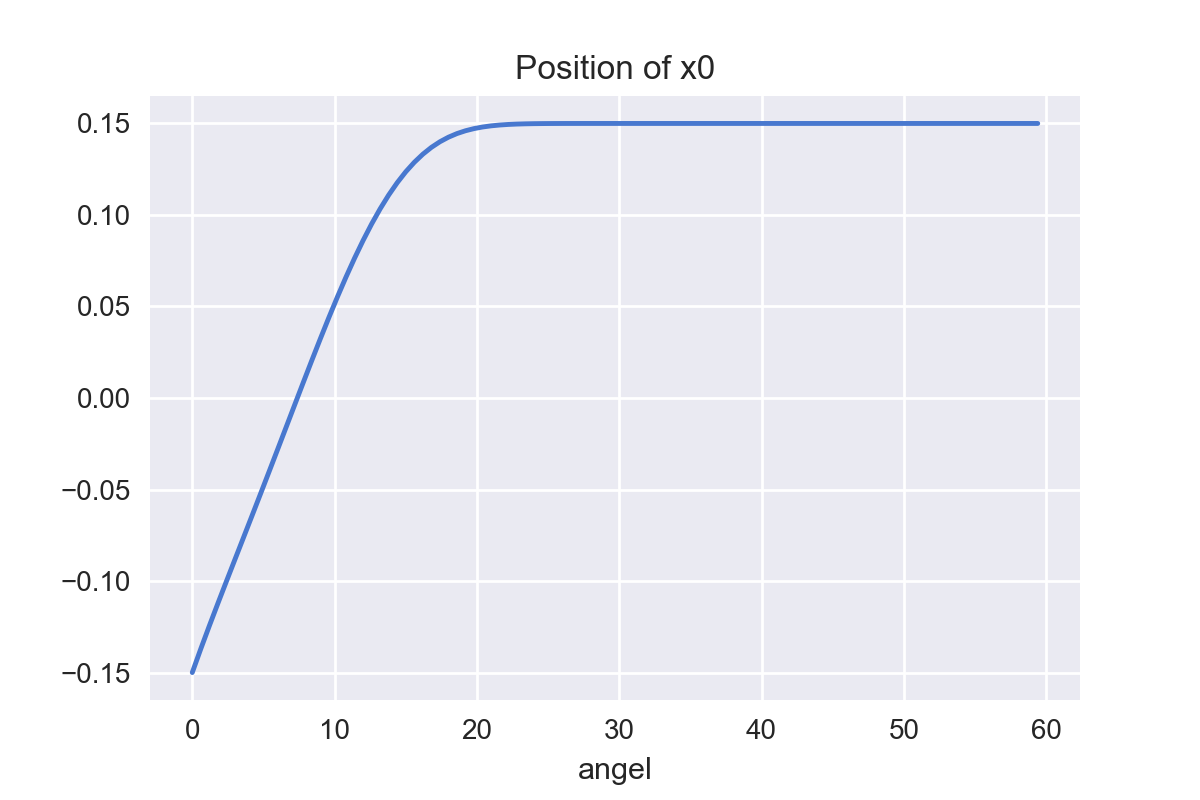
\includegraphics[width=\textwidth]{1-1.png}
\caption{临界侧向滑移点位置和侧偏角关系}
\label{fig:1-1}
\end{figure}
\begin{figure}[ht]
\centering
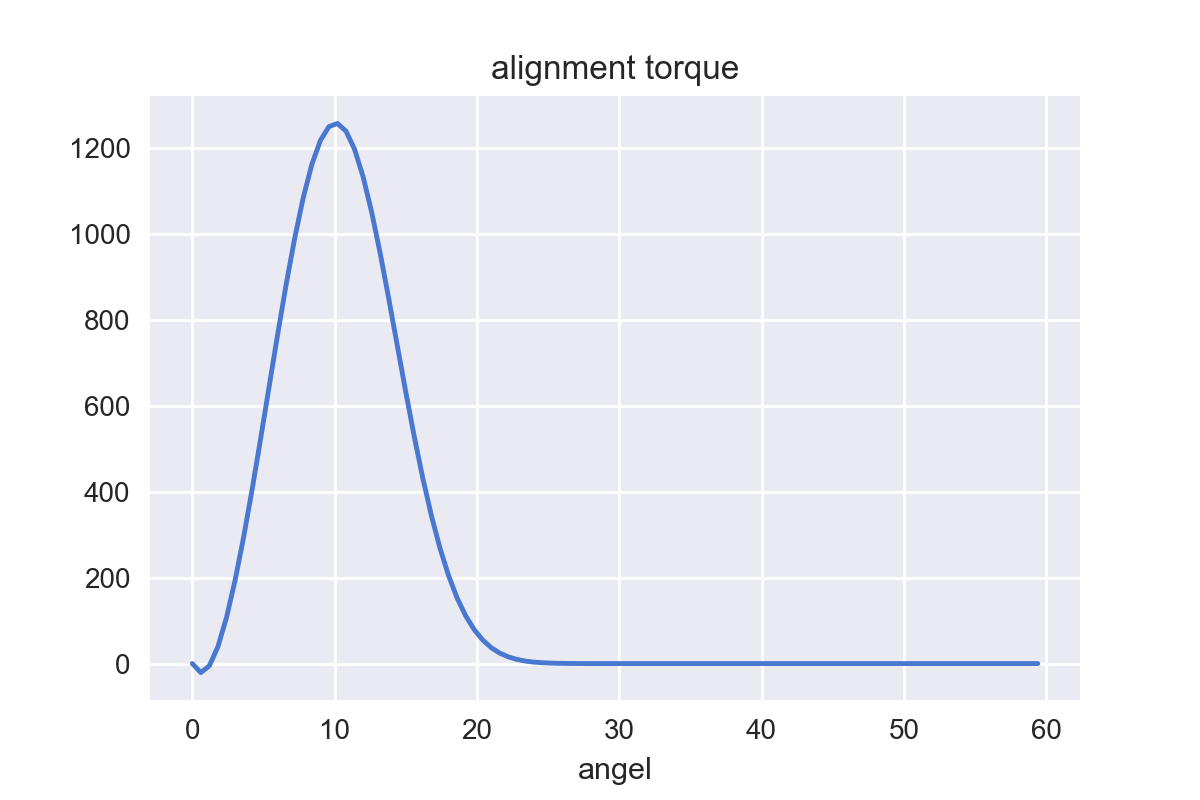
\includegraphics[width=\textwidth]{1-2.png}
\caption{回正力矩和侧偏角关系}
\label{fig:1-2}
\end{figure}
\subsection{(2)}
首先求解垂直力的分布,和(1)类似首先由
\begin{equation}
\int_{-\frac{l}{2}}^{\frac{l}{2}} P dx = F_z
\end{equation}
得
\begin{equation}
\label{eq:2.1}
F_z = al + \frac{b}
{12}l^3 - c \sin(\frac{2\pi x}{l})
\end{equation}
同时,在边缘处应该为力的零值边界条件,有
\begin{equation}
\label{eq:2.2}
P(-\frac{l}{2}) = 
P(\frac{l}{2})  = 0
\end{equation}
联立方程\ref{eq:2.1}和方程\ref{eq:2.2}可得
\begin{align*}
a & = \frac{3F_z}{2l}\\
b & = -\frac{6F_z}{l^3}
\end{align*}
那么载荷的垂直分布为
\begin{equation*}
\label{eq:p}
P = \frac{3F_z}{2l} -\frac{6F_z}{l^3}x^2- c \sin(\frac{2\pi x}{l})
\end{equation*}
有滚动阻力特性
\begin{equation}
\label{eq:f}
M_y = fRF_z = \int_{-\frac{l}{2}}^{\frac{l}{2}} Px dx
\end{equation}
将方程\ref{eq:f}代入方程\ref{eq:p}中可以求出
\begin{equation}
c = -\frac{2\pi fRF_z}{l^2}
\end{equation}
那么载荷的垂直分布求得
\begin{equation}
P = \frac{F_z}{2l^3}(3l^2 - 12x^2) + \frac{2\pi fRF_z}{l^2}sin(\frac{2\pi x}{l})
\end{equation}

为了求解侧向力的分布,假设其为简单的线性分布,即假设其方程为
\begin{equation}
f_y = k_y (x-\frac{l}{2})
\end{equation}
接下来就是求出这一分布和最大侧向力轮廓的交点(显然,从这一交点往印记后方,侧向李将会沿着最大侧向力轮廓分布),不妨设交点的横坐标为$x_0$,有
\begin{equation}
k_y (x_0-\frac{l}{2}) = \mu_y\left(\frac{3F_z}{2l} -y\frac{6F_z}{l^3}x_0^2 +\frac{2\pi fRF_z}{l^2}sin(\frac{2\pi x}{l})  \right)
\end{equation}
容易求得
\begin{equation}
k_y = \frac{\mu_y}{x_0 + l/2} \left( \frac{F_z}{2l^3}(3l^2 - 12x_0^2) + \frac{2\pi fRF_z}{l^2}sin(\frac{2\pi x}{l}) \right) 
\end{equation}
从而可以得到侧向力的分布
\begin{equation}
\label{eq:cepian}
f_y(x)=
\begin{cases}
k_y(x - \frac{l}{2})& \text{$x_0 \leq x \leq \frac{l}{2}$}\\
\mu_y P & \text{$-\frac{l}{2} \leq x \leq x_0$}
\end{cases}
\end{equation}
对侧向力的分布进行积分,可以得到总的侧向力
\begin{equation}
F_y = \int_{-\frac{l}{2}}^{\frac{l}{2}} f_y dx
\end{equation}
代入求得
\begin{equation}
\begin{split}
F_y = -\frac{k_y}{2}(x_0-\frac{l}{2})^2 + \frac{\mu_y F_z}{2l^3}(l^3+3l^2x_0-4x_0^3) \\ - \frac{\mu_y fRF_z}{l} \left(1 + \cos(\frac{2\pi x_0}{l}) \right) \\ -\frac{F_z\mu_y \pi fRl}{2l^3}(2x_0 - l)sin(\frac{2\pi x_0}{l})
\end{split}
\end{equation}
而题干中已知
\begin{equation}
F_y = \mu_y \times F_z \times \left[1-e^{-(\psi + E_y \times \psi^3)}\right]
\end{equation}
得到方程
\begin{equation} 
\label{eq:2.3}
\begin{split}
8x_0^3 -12lx_0^2 + 6l^2x_0 + l^3(8e^{-(\psi + E_y \times \psi^3)}-1) \\ -8fRl^2 \left(1+ \cos(\frac{2 \pi x_0}{l}) \right) \\-4\pi fRl(2x_0 -l)sin(\frac{2\pi x_0}{l}) = 0
\end{split}
\end{equation}
注意到
\begin{equation}
\label{eq:1.4}
\psi = \frac{K \times tg{\partial}}{\mu_y \times F_z}
\end{equation}
结合方程\ref{eq:1.3}和\ref{eq:1.4},可以将$x_0$表示为只和侧偏角$\partial$相关的函数,不妨记为$x_0 = \Psi(\partial)$

基于之前求得的侧向力公式\ref{eq:cepian},可以求出回正力矩为
\begin{equation}
\begin{split}
M_z = \int_{-\frac{l}{2}}^{\frac{l}{2}} f_y dx = \frac{u_yF_z}{2l^3}\left(x_0^4 -10lx_0^3 -\frac{9}{2}x_0^2 + \frac{5}{2}l^3x_0 + \frac{17}{16}l^4 \right) \\
+ \frac{\mu_y fRF_z}{l} \left(-\frac{l}{2} + \frac{l}{2\pi}sin(\frac{2\pi x_0}{l}) + x_0 cos(\frac{2\pi x_0}{l}) \right) \\
-\frac{\mu_y \pi fF_zR}{12l^2}(8x_0^2 - 2lx_0 - l^2)sin(\frac{2\pi x_0}{l})
\end{split}
\end{equation}
编写\textbf{Python}程序(见附录\ref{AppendixB}),特别地,采用牛顿迭代法进行方程求解,求解出临界侧向滑移点位置和回正力矩分别和侧偏角的关系如图\ref{fig:2-1}和图\ref{fig:2-2}所示
\begin{figure}[ht]
\centering
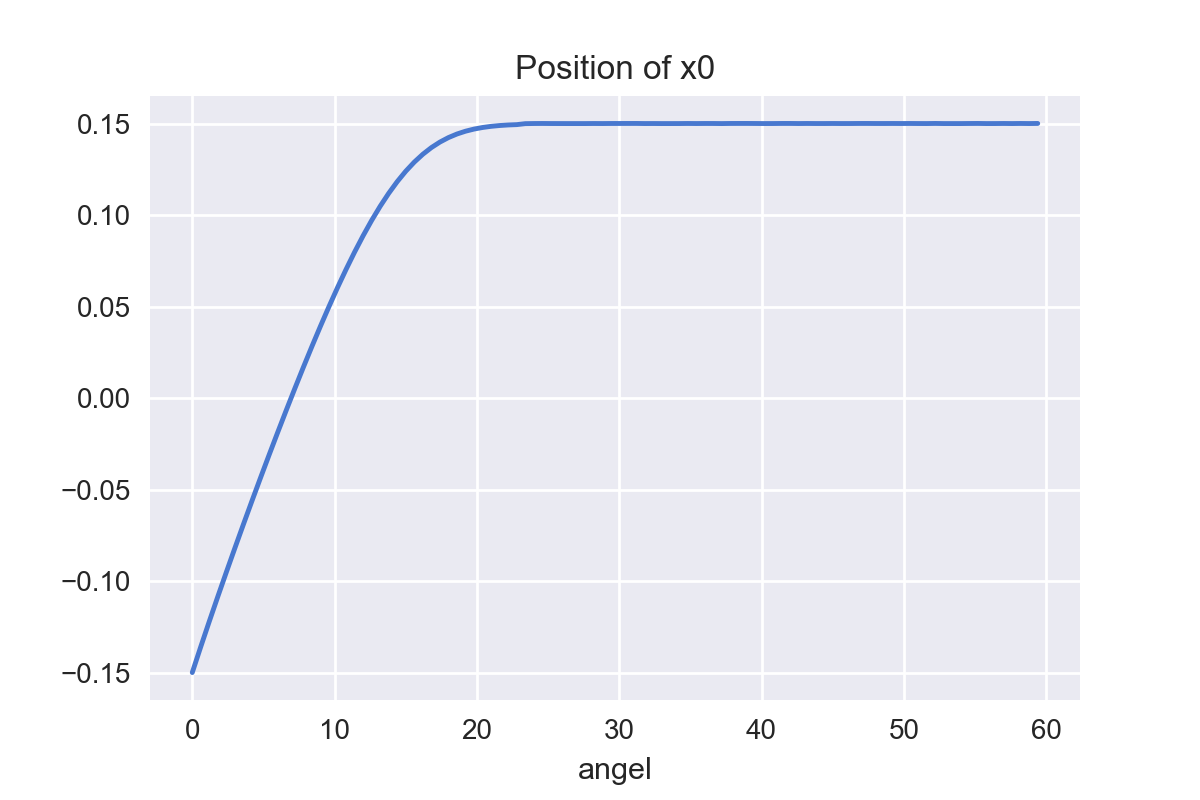
\includegraphics[width=\textwidth]{2-1.png}
\caption{临界侧向滑移点位置和侧偏角关系}
\label{fig:2-1}
\end{figure}
\begin{figure}[ht]
\centering
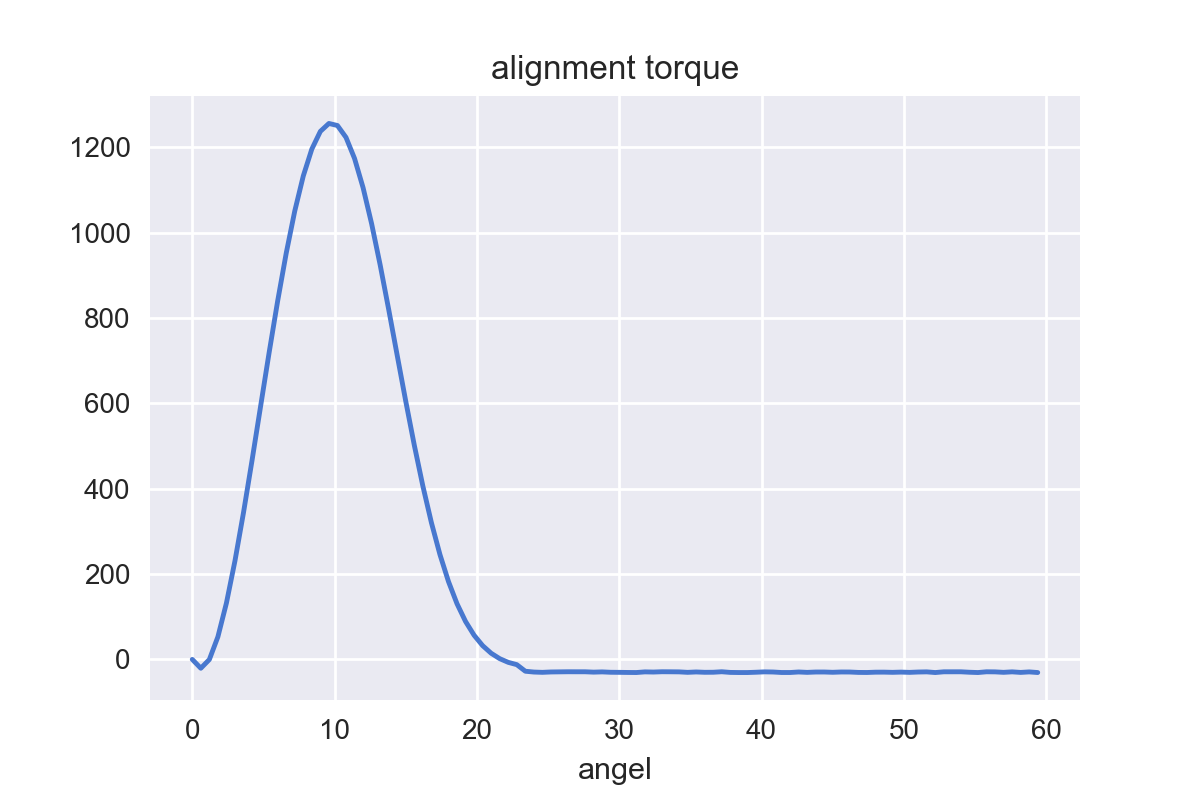
\includegraphics[width=\textwidth]{2-2.png}
\caption{回正力矩和侧偏角关系}
\label{fig:2-2}
\end{figure}
\section{Appendixs}
\subsection{AppendixA}
\label{AppendixA}
\begin{lstlisting}
# -*- coding: utf-8 -*-
"""
@author: feiyuxiao
"""
from sympy.solvers import solve
from sympy import Symbol
import math
import numpy as np
import matplotlib.pyplot as plt
import seaborn as sns

sns.set(style="darkgrid", palette="muted", color_codes=True)

x=Symbol('x')

k = 81000/(0.8*8000)
Ey = 0.1
l = 0.3
def g(rad):
    theta = k * math.tan(rad)
    return math.exp(-(theta+Ey*theta**3))

size = 100

kk = 0.8*8000/(2*l**3)
def M(x):
    return kk*(x**4 - 10*l*x**3 -4.5*l**2*x**2 + 2.5*l**3*x + 17*l**4/16)


angle = np.zeros(size)
angle_theta = np.zeros(size)
x0 = np.zeros(size)
M0 = np.zeros(size)

for i in range(size):
    angle[i] = i*(math.pi/(3*size))
    angle_theta[i] = 60*i/size

for i in range(size):    
    f =  8 * x**3 - 12*l*x**2 + 6*l*l*x + l*l*l*(g(angle[i])-1)
    s=solve(f, x)
    x0[i] = s[0]
    M0[i] = M(x0[i])
    
plt.figure()
plt.plot(angle_theta,x0)
plt.xlabel("angel")
plt.title("Position of x0")
plt.savefig("1-1.png",dpi=200)

plt.figure()
plt.plot(angle_theta,M0)
plt.xlabel("angel(rad)")
plt.title("alignment torque")
plt.savefig("1-2.png",dpi=200)   
\end{lstlisting}

\subsection{AppendixB}
\label{AppendixB}
\begin{lstlisting}
# -*- coding: utf-8 -*-
"""
@author: feiyuxiao
"""
import sympy
from sympy import Symbol
import math
import numpy as np
import matplotlib.pyplot as plt
import seaborn as sns
import random

pi = 3.1416
sns.set(style="darkgrid", palette="muted", color_codes=True)

x=Symbol('x')


k = 81000/(0.8*8000)
Ey = 0.1
l = 0.3
def g(rad):
    theta = k * math.tan(rad)
    return math.exp(-(theta+Ey*theta**3))

size = 100

kk1 = 0.8*8000/(2*l**3)
kk2 = 0.8*0.01*0.36*8000/0.3
kk3 = -0.8*pi*0.01*8000*0.36/(12*l*l)
def M(x):
    return kk1*(x**4 - 10*l*x**3 -4.5*l**2*x**2 + 2.5*l**3*x + 17*l**4/16) \
+ kk2*(-0.5*l + l*math.sin(2*pi*x/l)/(2*pi)+x*math.cos(2*pi*x/l)) \
+kk3*(8*x**2 -2*l*x -l*l)*math.sin(2*pi*x/l)


angle = np.zeros(size)
angle_theta = np.zeros(size)
x0 = np.zeros(size)
M0 = np.zeros(size)

for i in range(size):
    angle[i] = i*(pi/(3*size))
    angle_theta[i] = 60*i/size

F1 = -8*0.01*0.36*l*l
F2 = -4*pi*0.01*0.36*l
F0 = 2*pi/l

   
for i in range(size):    
    f =  8 * x**3 - 12*l*x**2 + 6*l*l*x + l*l*l*(8*g(angle[i])-1) \
    + F1*(1+sympy.cos(F0*x))  + F2*(2*x-l)*sympy.sin(F0*x)
    ffunc = sympy.diff(f, x)

    begin = 1
    end = 2
    
    MAXSTEP = 100
    
    step_count = 0
    
    xx0 = random.uniform(begin, end)
    temp = f.subs(x, xx0)
    
    while step_count < MAXSTEP and abs(temp) > 1e-10:
        xx0 = xx0 - (temp / (ffunc.subs(x, xx0)))
        temp = f.subs(x, xx0)
        step_count += 1
    x0[i] = xx0
    #print(step_count)
    M0[i] = M(x0[i])
    
plt.figure()
plt.plot(angle_theta,x0)
plt.xlabel("angel")
plt.title("Position of x0")
plt.savefig("2-1.png",dpi=200)

plt.figure()
plt.plot(angle_theta,M0)
plt.xlabel("angel")
plt.title("alignment torque")
plt.savefig("2-2.png",dpi=200)    
\end{lstlisting}
\end{document}